\section{Evaluation}
We evaluate \myds and Phoenix on 
a 32-core Intel 4× Xeon E7-4820 system equipped with 128GB of RAM. 
The operating system is Ubuntu 12.04 with kernel 3.2.0 and glibc-2.15.
Benchmarks were built as 64-bit executables with gcc -O3.
We logically disable CPU cores using Linux’s CPU hotplug mechanism, 
which allows to disable or enable individual CPU cores 
by writing “0” (or “1”) to 
a special pseudo file (/sys/devices/system/cpu/cpuN/online), 
and the total number of threads was matched to the number of CPU cores enabled.
Each workload is executed 10 times. 
To reduce the effect of outliers, 
the lowest and the highest runtimes for each workload are discarded, 
and thus each result is the average of the remaining 8 runs.

%\subsection{ Performance Improvements Summary}
\subsection{Performance of benchmarks}
%描述benchmarks的特点,benchmarks的数据集等

\begin{figure*}[htpb]
\centering
  \subfigure[SMR versus Phoenix with ptmalloc]{
   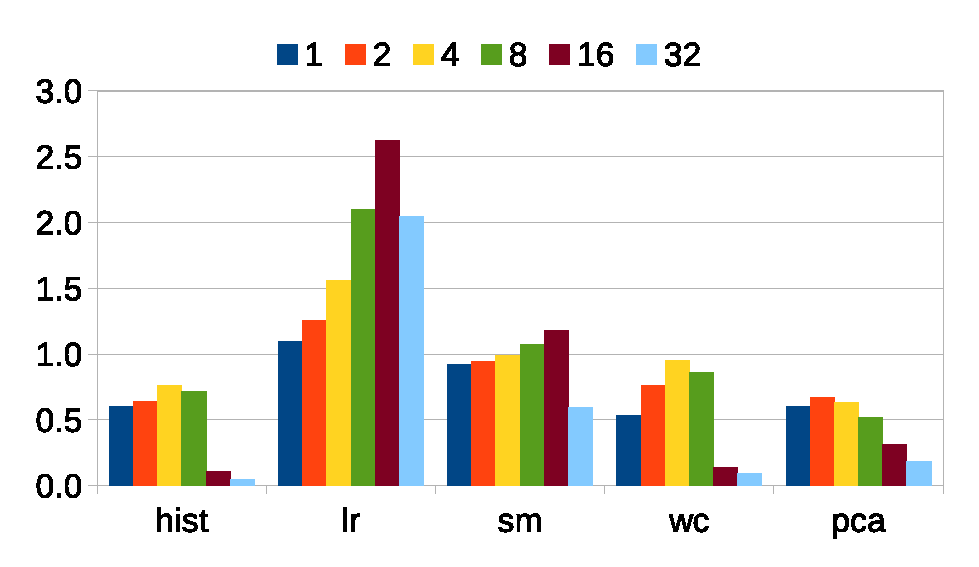
\includegraphics[width=0.45\textwidth]{eps/dmr_time_array.eps}
   \label{fig:dmr:time:ptmalloc}
  }
  \subfigure[SMR versus Phoenix with jemalloc]{
   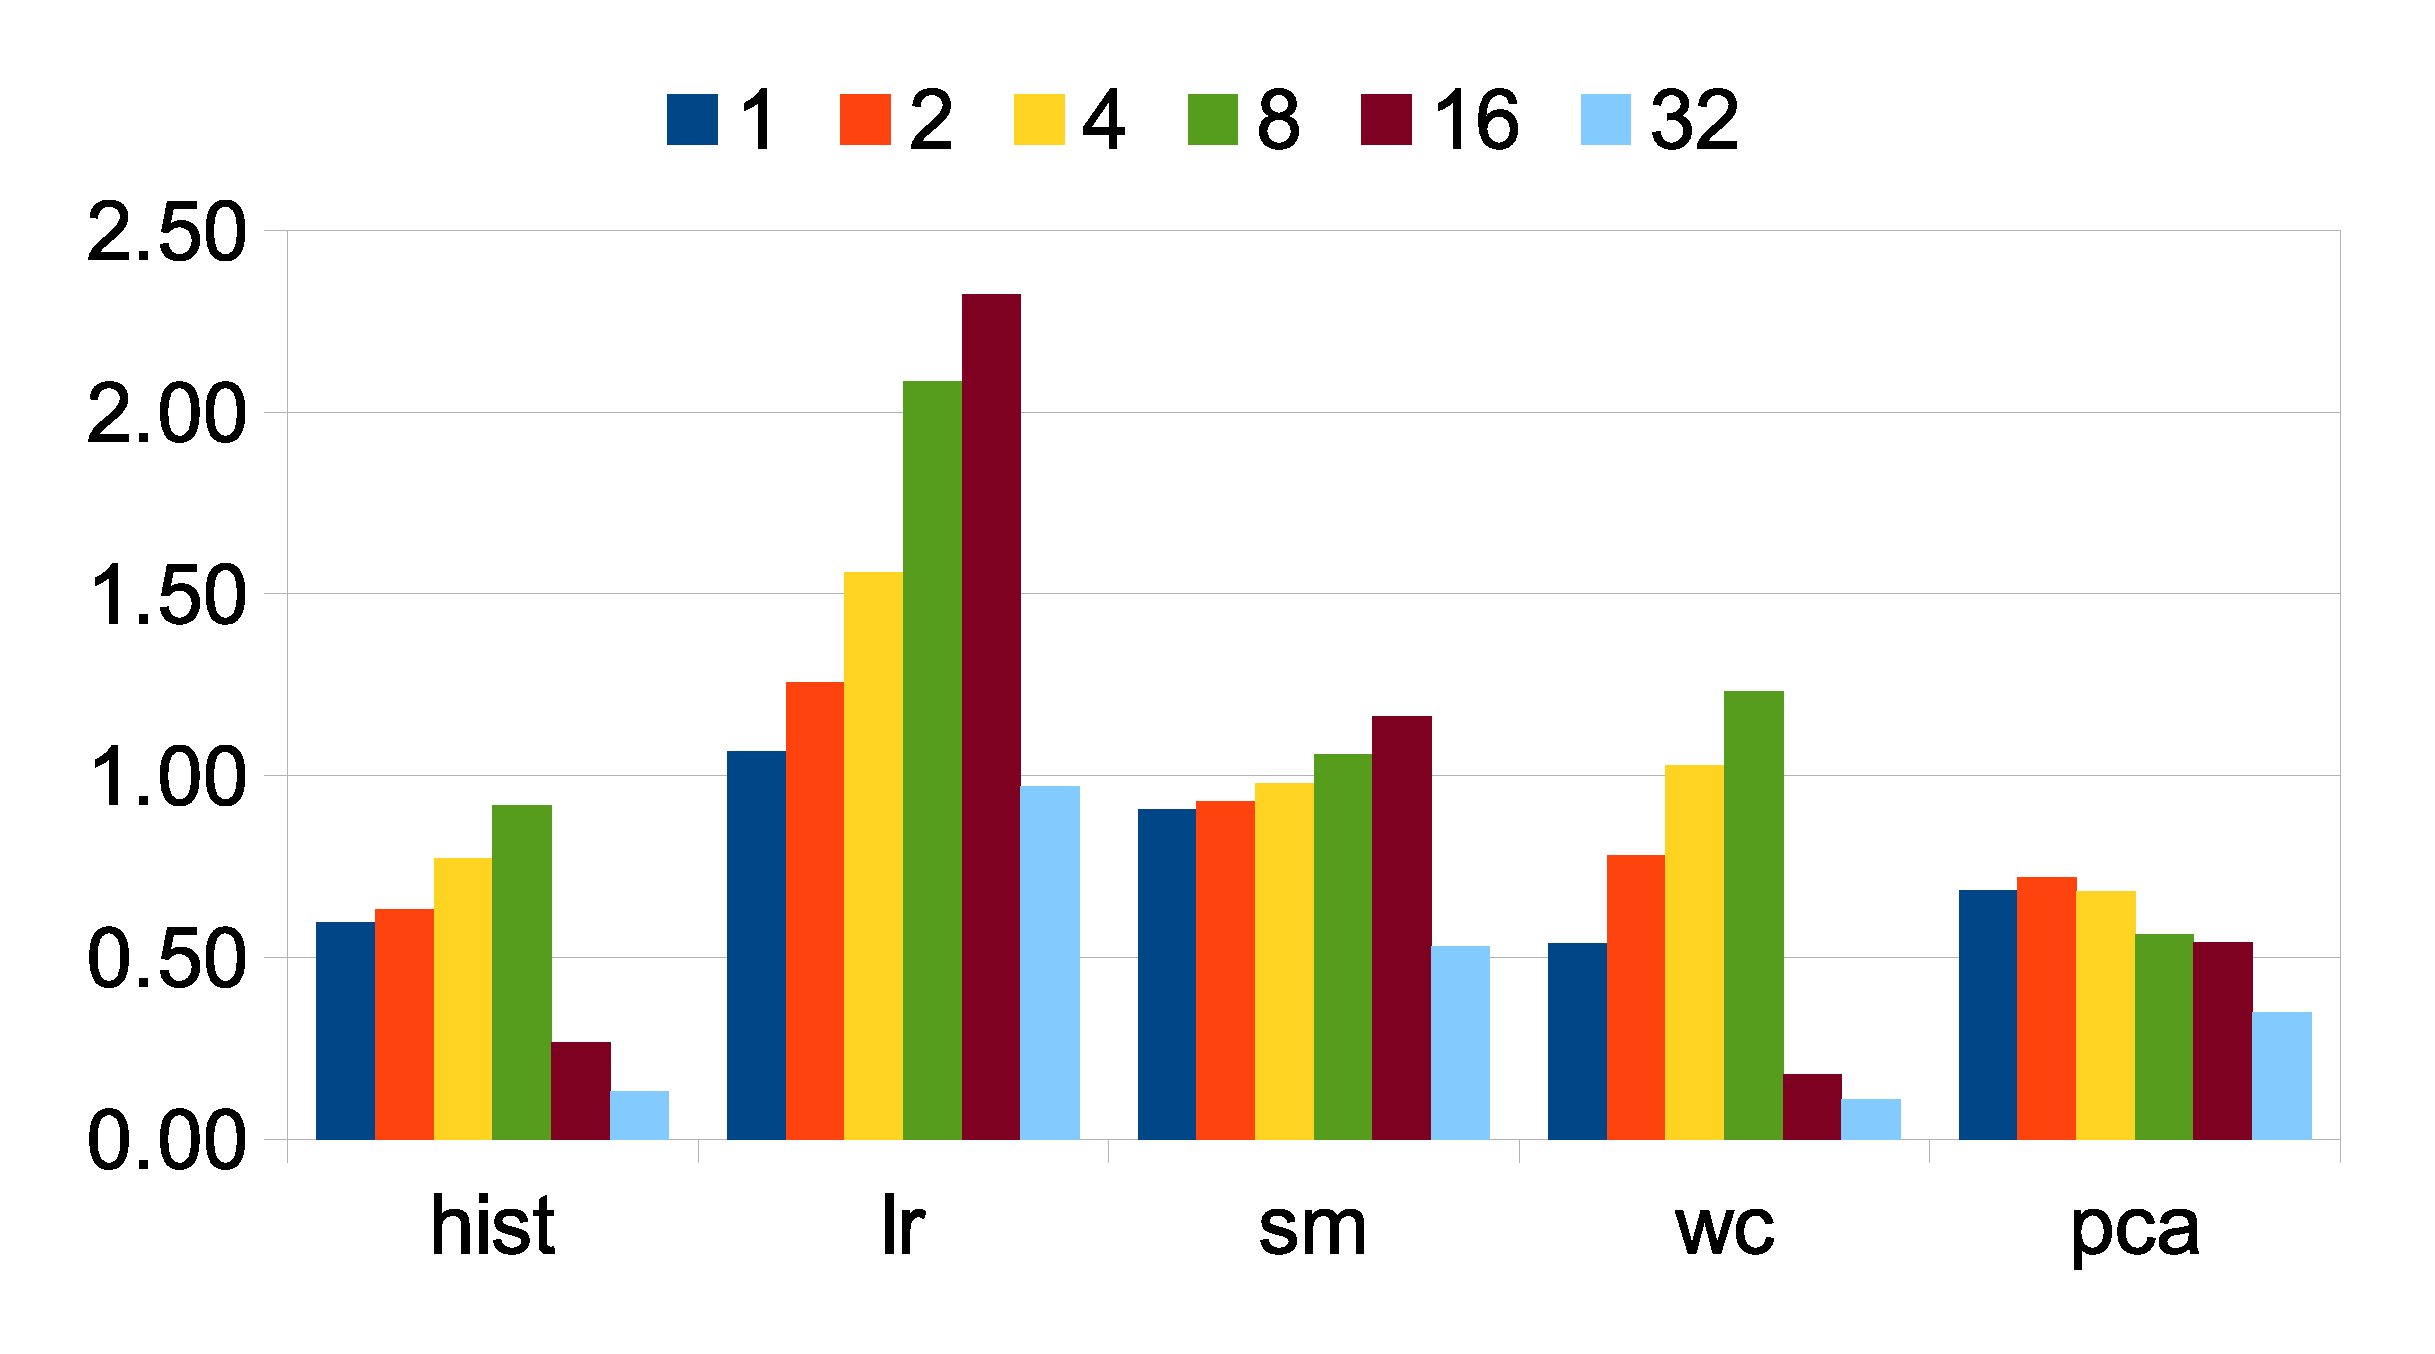
\includegraphics[width=0.45\textwidth]{eps/dmr_time_jemalloc.eps}
   \label{fig:dmr:time:jemalloc}
  }
  \caption{Execution time of SMR versus Phoenix}
   \label{fig:time}
\end{figure*}

{\bf Performance}
We measured \myds performance by executing the applications
included in the original release. 
\grayt{Table II describes the workloads and their input datasets. 
Compared to Phoenix, we significantly increased the performance.
However, some of the workloads still did not scale particularly well. 
We discuss their bottlenecks in detail in Section 5, 
but in the remainder of this section 
we first focus on the optimizations that turned out to be successful.
}
We experimented with various allocators.
Since there are many heap objects shared among threads
in Phoenix, and it is sensitive to memory allocator.
Compared to the libc sequential allocator ,  
ptmalloc\cite{gloger1997ptmalloc},
jemalloc{evans2006jemalloc} provided improved performance. 
the memory allocator in glibc, does not scale on multicore system. 
Therefore we evaluate the Phoenix with jemalloc and
compare it  with \myds(Figure \label{fig:dmr:time:jemalloc}).
Phoenix-jemalloc speedup Firgure \ref{fig:phoenix:speedup:jemalloc}

However, nether allocator could successfully scaled up to 32cores.

Figure\ref{fig:dmr:time:ptmalloc} and \ref{fig:dmr:time:jemalloc}
present the Execution time of \myds versus Phoenix.
%虽然jemalloc的性能表现要比ptmalloc好,但实验结果都显示
\myds matches or outperforms Phoenix on 4 out of 5 workloads,
but runs worse than Phoenix only on linear\_regression.
For hist, pca and word\_count, 
\myds outperforms Phoenix betwen xxx and xxx faster.
The reason of worse performance on linear\_regression 
is that most of time is waste in \myds's initailization.
We will evaluation overhead of initialization time in section\ref{}.
%从实验的结果可以看出,hist, wc, pca,SMR的性能较好,sm相当,lr中SMR的性能表现较差



\begin{figure*}[htpb]
\centering
  \subfigure[]{
   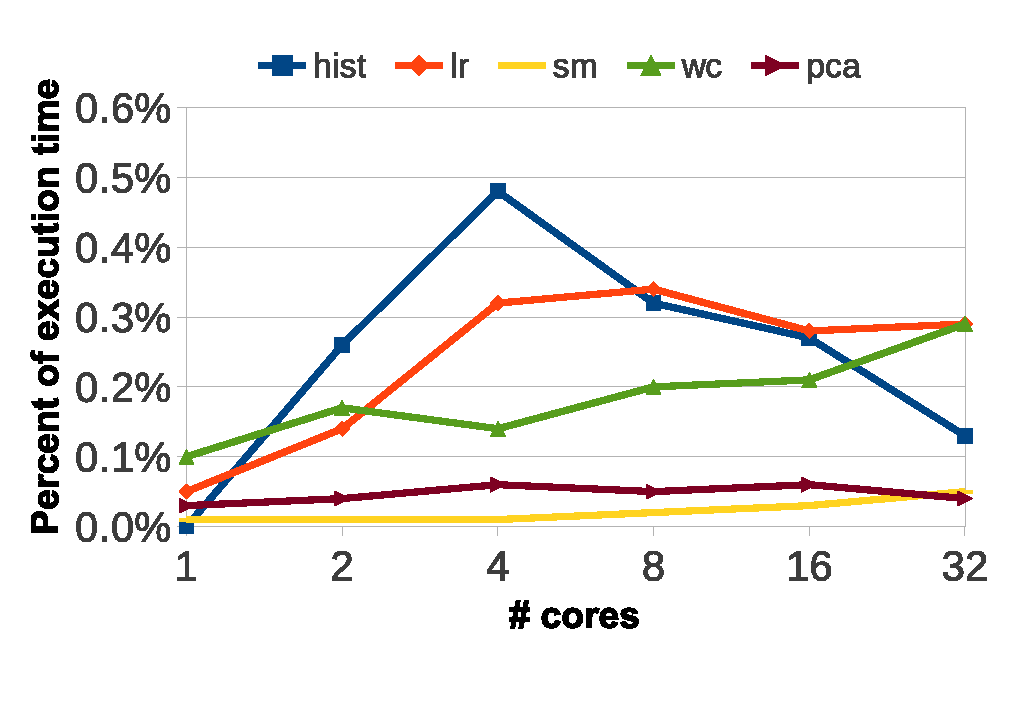
\includegraphics[width=0.45\textwidth]{eps/dmr_spinlock.eps}
   \label{fig:dmr:time:ptmalloc}
   }
  \subfigure[]{
   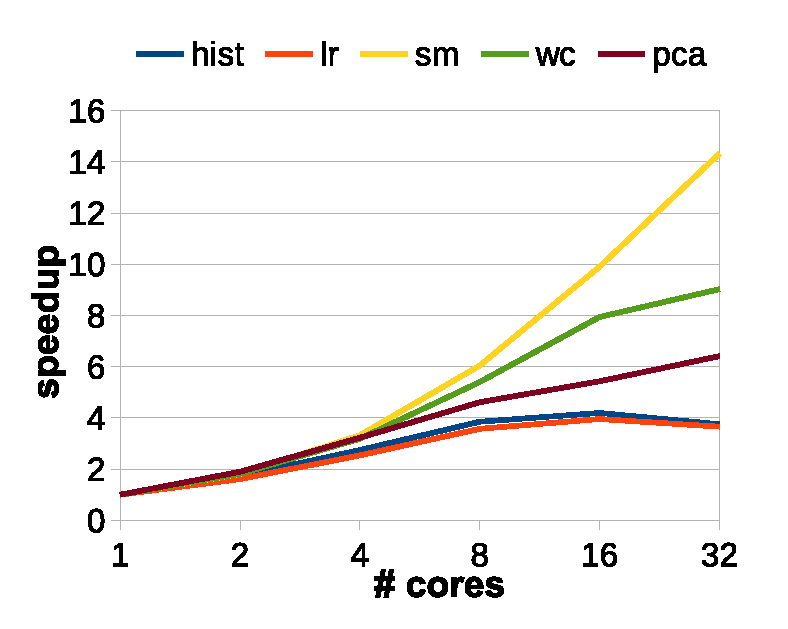
\includegraphics[width=0.45\textwidth]{eps/dmr_speedup.eps}
   \label{fig:dmr:time:jemalloc}
  }
  \caption{ Application speedup with the \myds}
   \label{fig:scalability}
\end{figure*}
{\bf Scalability}


We say a waiting thread is the thread which is waiting for shared
data that produced by another thread. If using semaphore for
synchronization, a waiting thread will be blocked and enlisted
on the waiting queue by the OS scheduler. If using spinlock
for synchronization, a waiting thread will do busy wait, i.e.
spinning in a while loop. Embedded software applications
that using semaphore to handle the synchronization could
result in performa+nce overkill, since it involves system calls
translated into thousands of CPU instructions [1]; while using
spinlock have problem of long busy-waiting time.

When a running thread tries to read shared data,
it must do busy wait until it has exhausted its time-slice
or until another thread has withdrawn the occupation on the
shared data. 




System performance is evaluated using
instructions per cycle (IPC). Higher IPC means
better performance.
Figure \ref{fig:perf:ipc} shows the IPC of Phoenix first increases 
and then decreases as more threads are run on multi-core system.


{\color{red}\myds }
Evaluation indicates that
the locking overhead can be significantly reduced to less
than 1% of total runtime on 32 cores




%分析lr性能差的原因

The performance of hist, wc, sm are scale linearly with the number of cores.


\subsection{ Impact of buffer Optimizations}
As the number of threads increases (from 1 to 8), the
execution time decreases for all cases. For 9 to 32 threads,
both Phoenix and \myds execution times keep decreasing with
the increase of the number of threads
When the number of dependent processes increases above the
number of cores, 
%context switching takes place, 
serious contending lock takes place,
and as a resultexecution time will be drastically increased. 
As the number of threads increases from 32 to 33, 
there is a significant increase
in execution time owing to Opteron’s NUMA architecture with
point-to-point communication links.

On the workstation, the \myds implementation is 13\%-
95\% better than Phoenix implementation (peaking at 8
threads).

As the number of threads increases (from 1 to 8), the
execution times for both Pthread/C and MPI programs decrease
for both workstation and supercomputer. For 9 threads to 32
threads, Pthread/C and MPI execution times changes slightly
on workstation. However for 9 threads to 32 threads, both
Pthread/C and MPI execution times keep decreasing (in most
cases) with the increase in number of threads on the
supercomputer node. This is because we use 8 cores in the
workstation while we use 32 cores in the supercomputer node.
Execution time for large number of threads (9 to 33 and
beyond) remains almost the same for the workstation because
of no communication overhead. Results (see Figure 4) also
show that MPI execution time on supercomputer increases
significantly when the number of threads is increased from 32
to 33 and beyond; but Pthread/C execution time on
supercomputer remains almost unchanged. This is due to the
communication overhead among the cores (32 cores in a
supercomputer node) when using MPI message passing.

From the
experimental results, it is observed that both computer systems
yield better performance using Pthread than MPI (in most
cases). Pthread has the advantage over MPI for sharing
memory and distributing tasks among lightweight threads
instead of processes. The performance of the Pthread
implementation on the supercomputer is the best, 30%-6.7x
better than the Open MPI implementation on the
supercomputer node.

\subsection{ Challenges and Limitations}
\begin{figure}[htpb]
\centering
  \subfigure[Execution time and initialization time on histgram]{
   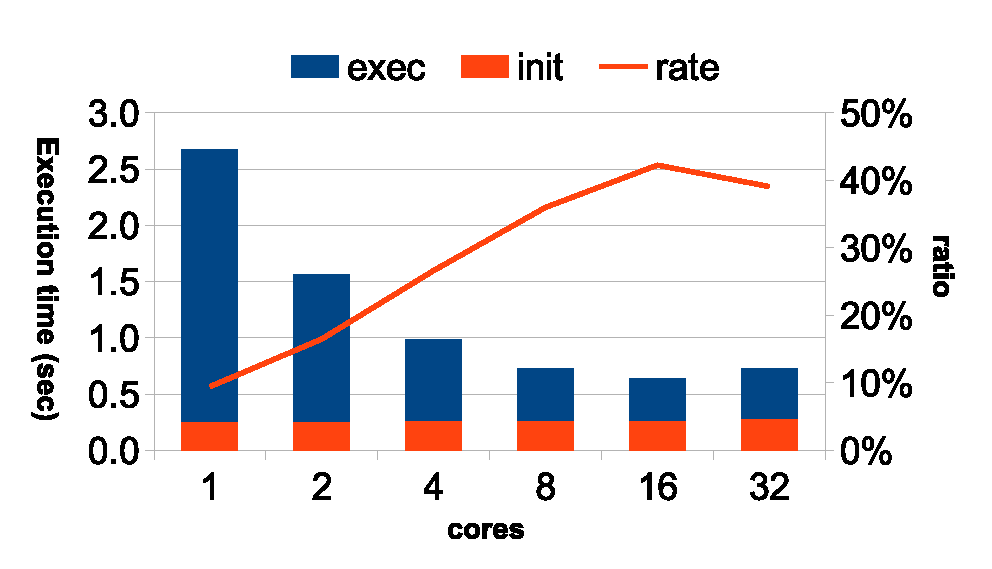
\includegraphics[width=0.45\textwidth]{eps/dmr_hist_init.eps}
   \label{fig:dmr:hist:init}
   }
  \subfigure[Execution time and initialization time on linear\_regression]{
   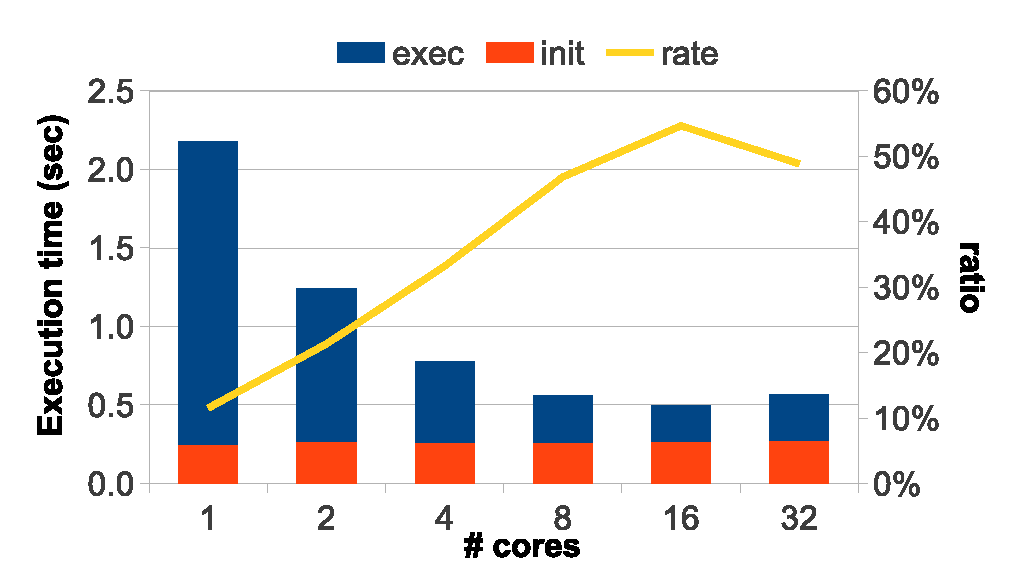
\includegraphics[width=0.45\textwidth]{eps/dmr_lr_init.eps}
   \label{fig:dmr:lr:init}
  }
  \caption{Initialize time with \myds}
   \label{fig:init}
\end{figure}
Figure\ref{fig:init} shows the initialization time of \myds and Phoenix.
The time of \myds used is range 0.25s to  0.35s, 
while it is just about 0.001s in Phoenix.
{\color{red} why the initialization time is so large in \myds}

Although we were able to significantly improve the scalability of \myds, 
workloads histogram, linear regression still did not scale up to 32cores. 
%We used /usr/bin/time to assess where the execution time was
We used stub to assess where the execution time was
being spent. 
Figure \ref{fig:dmr:hist:init} shows the result with exec time
defined as mapreduce actual execution time and init time as the initialization time before workers starting work. 
It was clear that the 2 non-scaling workloads shared two common trends. 
First, the init time ratio increased with increasing number of threads, 
dominating the total execution time at high thread count. 
%Second, the portion of actual computation time assumed by kernel code (sys /
%effective) significantly increased as we went beyond the single
%chip boundary.
%Second, both total execution time are short, While the portion of init time is 

\begin{figure}[htpb]
\centering
  \subfigure[]{
   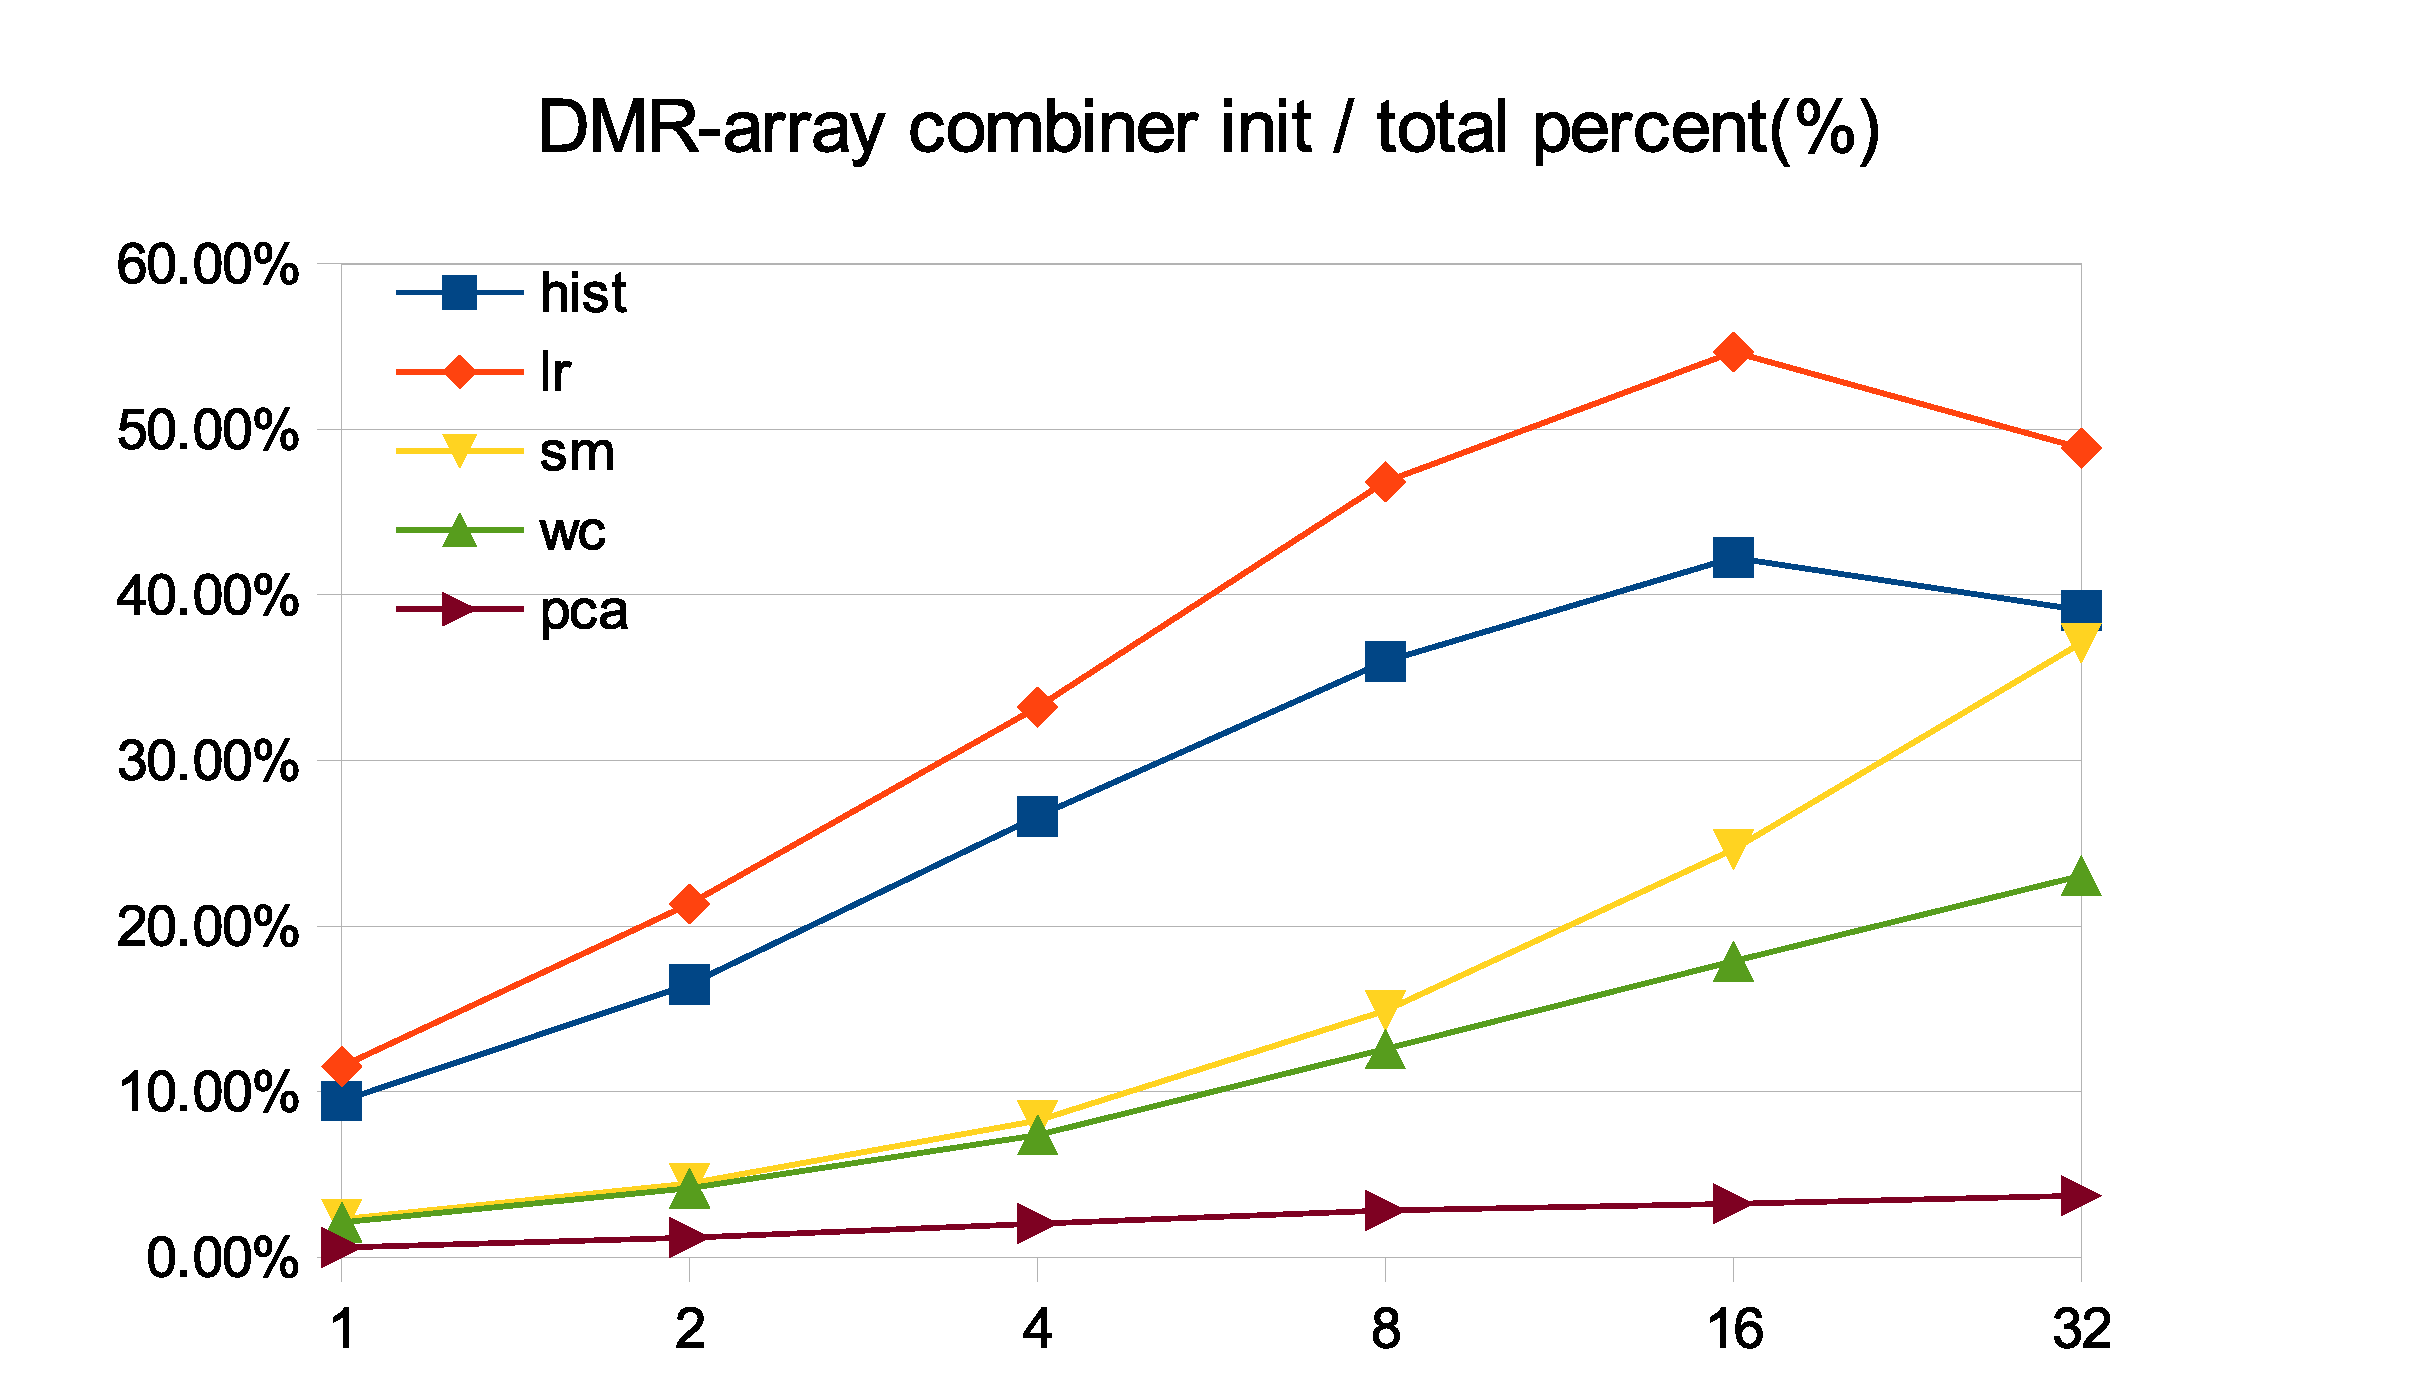
\includegraphics[width=0.4\textwidth]{eps/dmr_init.eps}
   \label{fig:dmr:time:jemalloc}
  }
  \caption{Initialize time of SMR and Phoenix}
   \label{fig:time}
\end{figure}

\redt{\myds initialization time is uesd to create threads, channel.}
%\myds的大部分时间用于了thread的创建,channel的分配,因此它的开销远大于Phoenix初始化的开销




